\section{Постановка задачи}

Исследование из области солнечной энергетики \cite{litlink1}. На рис. \ref{pic:scheme} показана схема установки для исследования фотоэлектрических характеристик.
\begin{figure}[H]
	\centering
	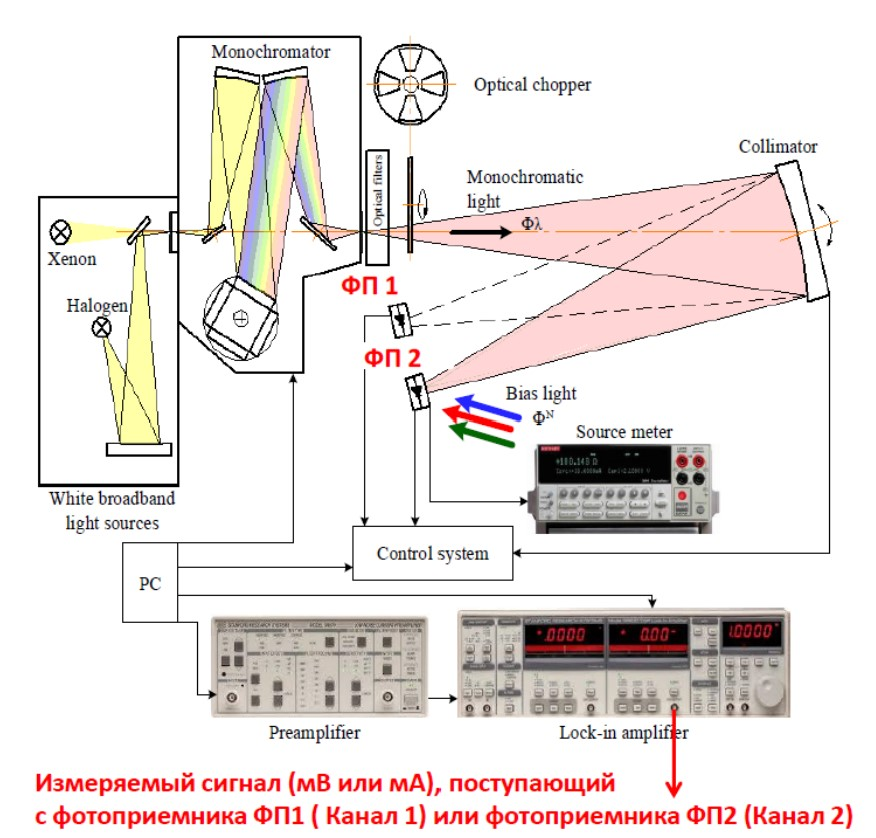
\includegraphics[scale=0.9]{resources/scheme.jpg}
	\caption{Схема установки}
	\label{pic:scheme}
\end{figure}

Калибровка датчика ФП1 производится по эталону ФП2. Зависимость между квантовыми эффективностями датчиков предполагается одинаковой для каждой пары измерений
\begin{equation}
	QE_{ФП2} = \frac{I_{ФП2}}{I_{ФП1}}*QE_{ФП1},
	\label{eq:quantum}
\end{equation}
где $QE_2, QE_1$ -- квантовые эффективности эталонного и исследуемого датчиков, $I_2, I_1$ -- измеренные токи. \\

\textbf{Исходные данные.}
Даны 2 выборки данных с интервальной неопределенностью. Одна из них относится к эталонному датчику ФП2, другая -- к исследуемому датчику ФП1.

\textbf{Задача.}
Требуется определить коэффициент калибровки
\begin{equation}
	R_{21} = \frac{I_{2}}{I_{1}}
	\label{eq:task}
\end{equation}
методом линейной регрессии на множестве интервальных данных и коэффициента Жаккара.

\newpage
